\documentclass{article}
\usepackage{graphicx}
\graphicspath{ {./images/} }
\title{Modelling with Graphs Summative }
\begin{document}
\maketitle
\newpage
\section*{A.3}
\subsection*{A.3.1}
To transform problem A.3 into a graph colouring problem , the problem is represented as a graph where:
\newline
Nodes = individual classes $(C_1,..., C_7)$
\newline
Edges = classes with at least one shared student (eg. "Amy" in $C_1$ and $C_5$)
\newline
Colour = A timeslot
\newline
\begin{center}
An example graph would be:
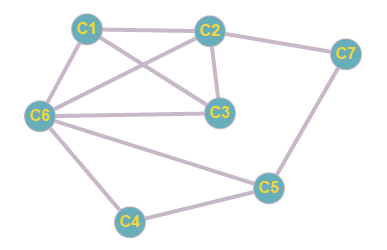
\includegraphics{a31NC}
\newline
\end{center}
The solution to the problem is the answer to the question, can the graph be coloured in at most 4 colours?
\newline
This will solve the problem because if the graph can be coloured so that no neighbouring nodes have the same timeslot then the student can physially attend every class, and by doing it in at most 4 colours means there are sufficient time slots.
\newline
An example colouring of the above graph would be:
\begin{center}
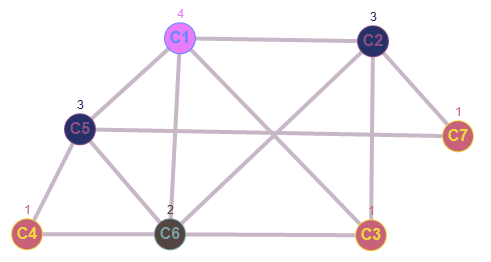
\includegraphics{a31C}
\end{center}
\end{document}